\documentclass{article}

%% PAQUETES

% Paquetes generales
\usepackage[margin=2cm, paperwidth=210mm, paperheight=297mm]{geometry}
\usepackage[spanish]{babel}
\usepackage[utf8]{inputenc}
\usepackage{gensymb}

% Paquetes para estilos
\usepackage{textcomp}
\usepackage{setspace}
\usepackage{colortbl}
\usepackage{color}
\usepackage{color}
\usepackage{upquote}
\usepackage{xcolor}
\usepackage{listings}
\usepackage{caption}
\usepackage[T1]{fontenc}
\usepackage[scaled]{beramono}

% Paquetes extras
\usepackage{amssymb}
\usepackage{float}
\usepackage{graphicx}
\usepackage{url}
\usepackage{enumerate}
\usepackage{color}

%% Fin PAQUETES


% Definición de preferencias para la impresión de código fuente.
%% Colores
\definecolor{gray99}{gray}{.99}
\definecolor{gray95}{gray}{.95}
\definecolor{gray75}{gray}{.75}
\definecolor{gray50}{gray}{.50}
\definecolor{keywords_blue}{rgb}{0.13,0.13,1}
\definecolor{comments_green}{rgb}{0,0.5,0}
\definecolor{strings_red}{rgb}{0.9,0,0}

%% Caja de código
\DeclareCaptionFont{white}{\color{white}}
\DeclareCaptionFont{style_labelfont}{\color{black}\textbf}
\DeclareCaptionFont{style_textfont}{\it\color{black}}
\DeclareCaptionFormat{listing}{\colorbox{gray95}{\parbox{16.78cm}{#1#2#3}}}
\captionsetup[lstlisting]{format=listing,labelfont=style_labelfont,textfont=style_textfont}

\lstset{
	aboveskip = {1.5\baselineskip},
	backgroundcolor = \color{gray99},
	basicstyle = \ttfamily\footnotesize,
	breakatwhitespace = true,   
	breaklines = true,
	captionpos = t,
	columns = fixed,
	commentstyle = \color{comments_green},
	escapeinside = {\%*}{*)}, 
	extendedchars = true,
	frame = lines,
	keywordstyle = \color{keywords_blue}\bfseries,
	language = Oz,                       
	numbers = left,
	numbersep = 5pt,
	numberstyle = \tiny\ttfamily\color{gray50},
	prebreak = \raisebox{0ex}[0ex][0ex]{\ensuremath{\hookleftarrow}},
	rulecolor = \color{gray75},
	showspaces = false,
	showstringspaces = false, 
	showtabs = false,
	stepnumber = 1,
	stringstyle = \color{strings_red},                                    
	tabsize = 2,
	title = \null, % Default value: title=\lstname
	upquote = true,                  
}

%% FIGURAS
\captionsetup[figure]{labelfont=bf,textfont=it}
%% TABLAS
\captionsetup[table]{labelfont=bf,textfont=it}

% COMANDOS

%% Titulo de las cajas de código
\renewcommand{\lstlistingname}{Código}
%% Titulo de las figuras
\renewcommand{\figurename}{Figura}
%% Titulo de las tablas
\renewcommand{\tablename}{Tabla}
%% Referencia a los códigos
\newcommand{\refcode}[1]{\textit{Código \ref{#1}}}
%% Referencia a las imagenes
\newcommand{\refimage}[1]{\textit{Imagen \ref{#1}}}


\begin{document}
\pagenumbering{roman}
\setcounter{page}{5}



% TÍTULO, AUTORES Y FECHA
\begin{titlepage}
	\vspace*{\fill}
	\begin{center}
		\Large 75.42 Taller de Programación I \\
		\Huge TP N°5: Archivos Ubicuos \\
		\bigskip\huge\textit{Grupo 04} \\
		\bigskip\bigskip\bigskip\bigskip\bigskip\bigskip
		\bigskip\bigskip\bigskip\bigskip\bigskip\bigskip\bigskip
		\medskip\huge\textit{``Documentación Técnica''} \\
		\date{}
	\end{center}
	\vspace*{\fill}
\end{titlepage}
\newpage




% ÍNDICE
\tableofcontents
\newpage
\pagenumbering{arabic}




% REQUERIMIENTOS DE SOFTWARE
\section{Requerimientos de software}
	
	Se listan a continuación los distintos requerimientos mínimos y necesarios para poder compilar, desarrollar, probar y depurar las aplicaciones que conforman al proyecto:
	\medskip

	\begin{itemize}
	\itemsep=5pt \topsep=0pt \partopsep=0pt \parskip=0pt \parsep=0pt

		\item \textit{Sistemas operativos}: GNU/Linux (x86 y x86-64, distribuciones Linux basadas en RPM y DEB);

		\item \textit{Controlador de versiones}\footnote{Este requerimiento es de caracter opcional ya que solo es necesario en caso de desear clonar el proyecto desde el repositorio del grupo.}: GIT (\url{http://git-scm.com/});

		\item \textit{Compilador}: g++ (\url{http://gcc.gnu.org/});

		\item \textit{Herramientas}: Make (\url{http://www.gnu.org/software/make/}).

	\end{itemize}
\bigskip




% DESCRIPCIÓN GENERAL
\section{Descripción general}

	El proyecto se encuentra dividido en tres aplicaciones principales: \textit{cliente}, \textit{servidor} y \textit{monitor}. El corazón central del servicio se encuentra establecido sobre el servidor, ya que las demás aplicaciones tienen como tarea mantenerse en contacto con este. Tal comunicación se realiza a travéz de sockets, permitiéndose así la ejecución remota de los programas, instanciados en distintos equipos.
	\par
	Para lograr tal fin, se han identificado ciertos módulos que dotarán de distintos tipos de funcionalidades a nuestras aplicaciones. Además de ello, y no menos importante, se establecerá la existencia de un protocolo conocido por los tres entes, de manera de poder entenderse entre si. Cabe señalar que la aplicación monitor no es capaz de interactuar con la aplicación cliente, sino que simplemente todas interactuan con el servidor.
\bigskip




% APLICACIÓN SERVIDOR
\section{Aplicación \textit{Servidor}}

	Al ser la parte central y motor del servicio, el servidor deberá constar de un conjunto de módulos los cuales permitirán dividir las distintas ocupaciones y eventos que deben atenderse en este.
	\par
	Como avance de lo que será la explicación detallada del propósito a cumplir por cada clase, veamos los tipos de eventos y como son manejados a grandes razgos por el servidor.
	\par
	En primer lugar, el servidor atenderá conexiones entrantes. Estas últimas son derivadas a un ente que se encargará de mantener una interacción con el cliente que se encuentra al otro lado del canal de comunicación. El primer paso que se realiza con este usuario es el inicio de sesión. Esto le permitirá identificarse y ser derivado de acuerdo a la credencial (nombre de usuario) presentada. 
	\par
	Cada usuario se encuentra vinculado a un ente que denomiaremos \textit{carpeta}. Al producirse una conexión entrante, cada usuario es derivado a la carpeta que le corresponde, agrupándose así en cada uno de los directorios las conexiones vinculadas a un mismo nombre de usuario.
	\par
	Llegado a este paso, es decir, una vez que una conexión es derivada a la carpeta correspondiente, se inicia la sincronización con el host de dicha comunicación. Esto se logra a través del intercamboo de mensajes los cuales llegan a cada ente que representa una conexion, y los cuales son todos depositados en un ente \textit{receptor}.
	\par
	Cada carpeta posee un módulo \textit{sincronizador} el cual se ocupa de tomar uno a uno los mensajes provenientes del receptor, los procesa y da la orden de realizar una acción en base a esto último. Entre estas acciones se encuentran: recibir un archivo, recibir una notificación de archivo eliminado, recibir partes correspondientes a un archivo modificado, etc.
	\par
	Al llegar un mensaje que solicita agregar un archivo, modificarlo o eliminarlo, se deriva con dicha notificación en el módulo \textit{manejador de archivos}, quien se encarga de lidiar con los archivos físicos.
\bigskip



% APLICACIÓN SERVIDOR - Clases
\subsection{Clases}

	Pasaremos ahora a detallar las clases que conforman el conjunto de módulos de la aplicación servidor. Se recomienda al lector que a medida que avance en cada descripción, visualice en los diagramas de clases mostrados posteriormente ya que esto sumará en el entendimiento de como es que se relacionan entre sí los entes.

	\begin{itemize}
	\itemsep=5pt \topsep=0pt \partopsep=0pt \parskip=0pt \parsep=0pt

		\item \textit{Servidor}: es la encargada de estar a la escucha de nuevas conexiones y de derivarlas a ConexionCliente;

		\item \textit{ConexionCliente}: primeramente se ocupa de que el usuario se identifique mediante el inicio de sesión. De ser válidado correctamente este último, se deriva al objeto de ConexionCliente pertenenciente a dicha comunicación hacia el AdministradorDeClientes. En caso de no ser válido el inicio de sesión, la conexión se auto destruye;

		\item \textit{AdministradorDeClientes}: su tarea se limita a derivar a los clientes a sus respectivas carpetas lógicas, como así también es quien recibe las ordenes de dar de baja a un cliente de una carpeta y destruirlo;

		\item \textit{Validador}: es quien se encarga de validar los datos que envía el usuario para iniciar sesión en su carpeta;

		\item \textit{Carpeta}: los objetos de esta clase son administrados por AdministradorDeClientes. Estas representan la carpeta a nivel lógico de cada usuario. El Administrador se encarga de crear una sola de estas carpetas para un grupo de conexiones que se han loggeado con el mismo nombre de usuario. Cada carpeta posee asociado un conjunto de modulos con los cuales realizará emisiones y recepciones hacia los distintos objetos ConexionCliente de la carpeta, sincronizará y procesará mensajes entrantes y salientes y realizará el manejo de los archivos fisicos de la carpeta sobre el servidor. Las clases que representan estos módulos son: \textit{Actualizador}, \textit{Receptor}, \textit{Emisor}, \textit{Sincronizador} y \textit{ManejadorDeArchivos}.

	\end{itemize}

\bigskip



% APLICACIÓN SERVIDOR - Diagramas UML
\subsection{Diagramas UML}

	En la \textit{Figura 1} se muestra un diagrama de clases del corazón del servidor. En este se pueden notar las relaciones que hacen posible la derivación de un cliente hacia una carpeta una vez iniciada la sesión.
	
% Figura 1
\begin{figure}[h]
	\centering
	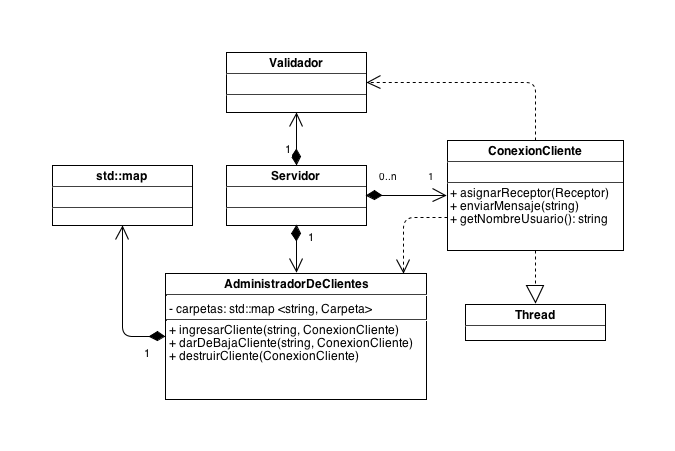
\includegraphics[width=0.85\textwidth]{images/Diagrama-modelo-servidor-parte1.png}
	\caption{Diagrama de clases principal del servidor.}
\end{figure}
\bigskip

\newpage

% Figura 2
\begin{figure}[h]
	\centering
	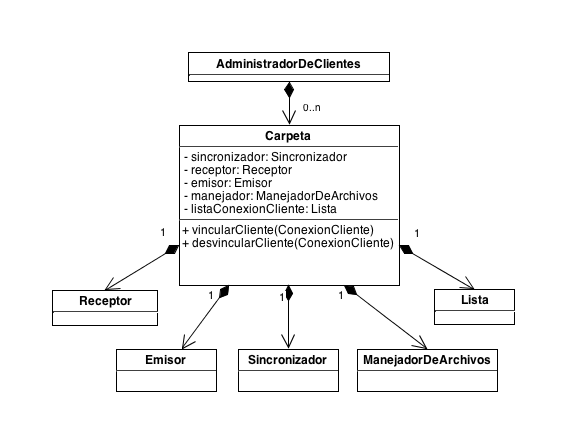
\includegraphics[width=0.72\textwidth]{images/Diagrama-modelo-servidor-parte2.png}
	\caption{Diagrama que muestra la jerarquía de clases principales.}
\end{figure}
\bigskip


% Figura 3
\begin{figure}[h]
	\centering
	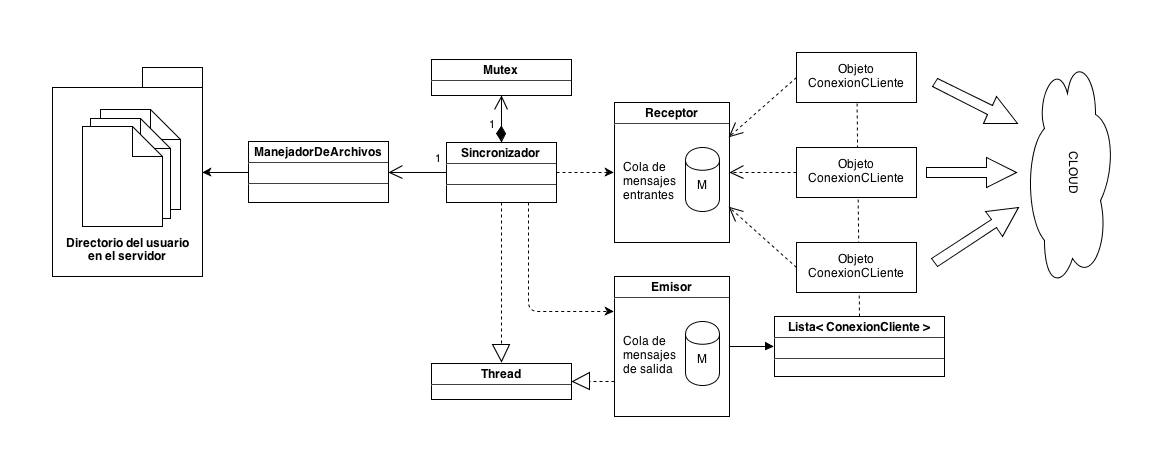
\includegraphics[width=1.0\textwidth]{images/Diagrama-modelo-servidor-parte3.png}
	\caption{Diagrama de representación de una Carpeta\\ con clientes conectados.}
\end{figure}
\bigskip






% APLICACIÓN SERVIDOR - Descripción de archivos  protocolos
\subsection{Descripción de archivos  protocolos}

	[ Colocar texto aquí ]
\bigskip




% APLICACIÓN CLIENTE
\section{Aplicación \textit{Cliente}}

	La aplicación cliente, consta de dos partes fundamentales: una que es desde el inicio de sesión hasta el proceso de actualización inicial, y la segunda es desde esa actualización inicial hasta el proceso de inspección general que se repite. 
	\par
	En la parte de actualización, las clases involucradas son Cliente, Receptor, Emisor, Manejador de Archivos y Actualizador. Lo primero que se realiza es la comparación entre lo que se encuentra en el registro de archivos \textit{.reg_archivos} con la lista de archivos que proviene del server. Se compara archivo por archivo en ManejadorDeArchivos y orquestrado por Actualizador, detectando bajas y modificaciones, y pidiendo uno a uno hasta que la información del servidor sea igual a la que se tiene en cliente. Los archivos nuevos que el cliente haya agregado offline, no serán tomados en cuenta en esta parte del proceso, pero sí lo serán los modificados offline, y se revertiran los cambios dejando como válida la copia que se encuentra en el servidor.
	\par
	Luego, finalizando la actualización, se inicia el proceso de inspección, en el cual se detectan los cambios que hayan en el directorio a partir de la base inicial que se estableció en el proceso anterior. Para esta parte, se hace uso de la clases Inspector y Sincronizador, que son las principales encargadas, junto con la ayuda de ManejadorDeArchivos, de lograr la sincronización correcta entre el cliente y el servidor. 
	Inspector se encarga de, como su nombre lo indica, ir comparando el registro \textit{.reg_archivos} (que es una copia fiel de la información que se encuentra actualmente en el servidor), con la lista de archivos que realmente se encuentra en el directorio a ser sincronizado por el cliente. Se realiza una inspección cada cierto intervalo de tiempo, en busca de cambios. Si encuentra alguno, se envian al servidor los bloques modificados (en el caso de que se trate de una modificación de un archivo existente), se envian los archivos nuevos detectados (en caso de tratarse de una alta) o se envia una notificación de eliminación de los archivos en el server (en caso de tratarse de una baja). 
	\par
	En ambos procesos, puede ocurrir que haya algún otro cliente conectado, que realice algún cambio sobre los archivos en el servidor. En tal caso, las modificaciones de este otro cliente, generan un mensaje que es enviado a los demás clientes conectados con la misma cuenta para que comparen su archivo actual con el que que se recibió, así pueden pedir las actualizaciones. Como puede que ocurran cambios de este estilo durante la actualización, se optó por analizar estos mensajes enviados a todos los clientes en este proceso de actualización también.
\bigskip



% APLICACIÓN CLIENTE - Clases
\subsection{Clases}

	La clase principal en cliente es \textit{Cliente}, que es la que se encarga de ser el puente entre la interfaz y el modelo, además de oquestrar el cambio del proceso de actualización al proceso de inspección. 
	\par
	Para realizar las sincronizaciones de archivos y controlar el manejo de información que fluye entre el cliente y el servidor, se hace uso de las clases \textit{Emisor} y \textit{Receptor}. Ambas contienen una cola de salida/entrada respectivamente de mensajes a ser intercambiados entre el servidor y el cliente. 
	\par
	Para el manejo de altas, bajas y modificaciones de archivos se hace uso de la clase \textit{Manejador de Archivos}, que se encarga de proveer una interfaz para las modificaciones de los archivos físicos en disco y provee además un mecanismo de detección de cambios en el directorio. Es la encargada de tratar a los archivos de a bloques, de comparar los hash correspondientes y de actualizar el \textit{.reg_archivos} cuando sea necesario. 
	\par
	La clase \textit{Manejador de notificaciones} es la que obtiene los mensajes desde el \textit{Receptor} y decide si es una notificacion para ser enviada directamente a \textit{Inspector} o si es un archivo, que debe ser procesado por \textit{Receptor de Archivos}. 
	\par
	La clase \textit{Inspector}, que ya fue explicada más arriba, es la encargada de procesar los cambios que hay en el directorio local contra la lista de archivos que se encuentran en el servidor. Esta es la que contiene la lógica para realizar la sincronización entre el servidor y el cliente. Utiliza a la clase \textit{Sincronizaddor}, que se ocupa de implementar los métodos necesarios, utilizando el protocolo establecido para intercambio de archivos.
	\par
	La clase \textit{Actualizador}, también explicada mas arriba y que solamente tiene vida durante el proceso de actualización, se encarga de dejar una copia estable de lo que se encuentra en el servidor, localmente. Los cambios offline, se tratan como casos especiales. 
\bigskip



% APLICACIÓN CLIENTE - Diagramas UML
\subsection{Diagramas UML}


% Figura 4
\begin{figure}[h]
	\centering
	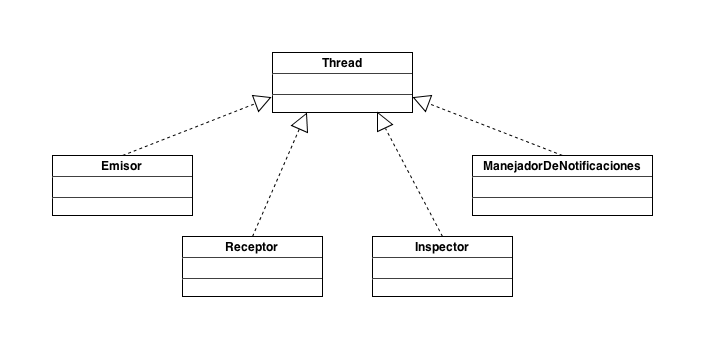
\includegraphics[width=0.85\textwidth]{images/Diagrama-modelo-cliente-threads.png}
	\caption{Diagrama de clases que indica aquellas que son un Thread.}
\end{figure}
\bigskip


% Figura 5
\begin{figure}[h]
	\centering
	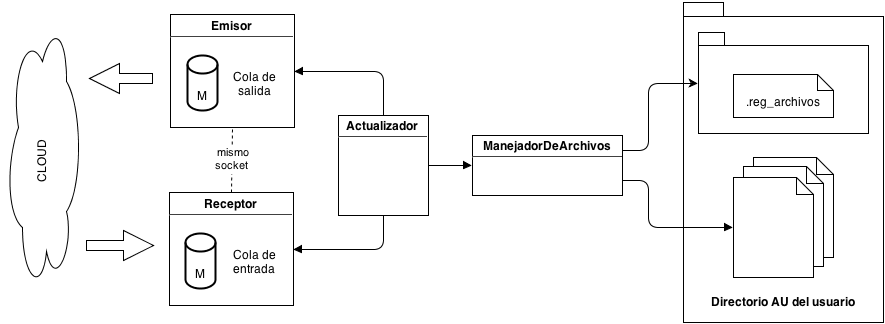
\includegraphics[width=1.0\textwidth]{images/Diagrama-modelo-cliente-actualizacion.png}
	\medskip
	\caption{Diagrama de clases que muestra de que forma se \\ relacionan en el proceso de actualización inicial.}
\end{figure}
\bigskip


% Figura 6
\begin{figure}[h]
	\centering
	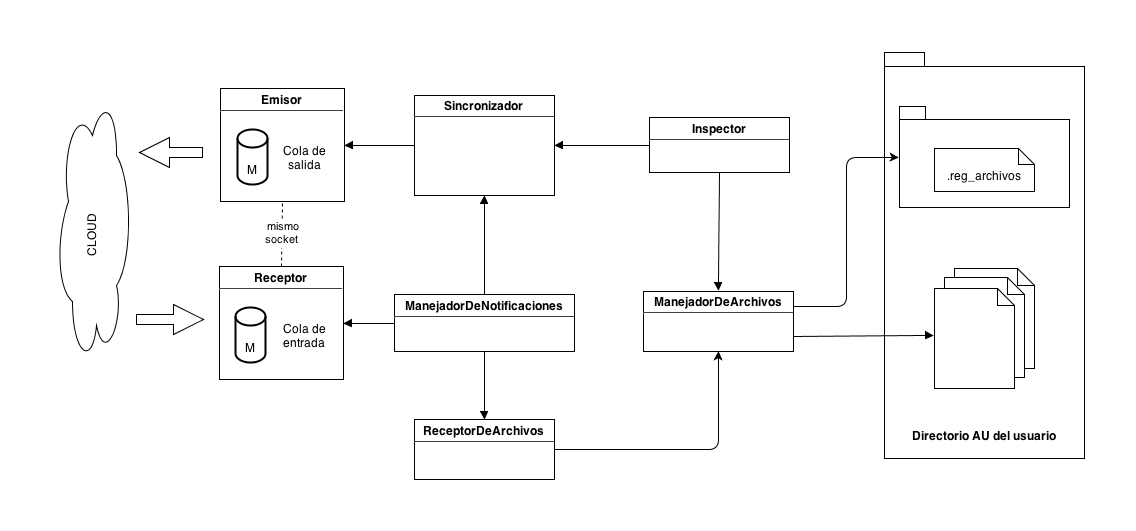
\includegraphics[width=1.0\textwidth]{images/Diagrama-modelo-cliente.png}
	\caption{Diagrama de clases que muestra de que forma se \\ relacionan en el proceso de sincronizacion.}
\end{figure}
\bigskip



% APLICACIÓN CLIENTE - Descripción de archivos  protocolos
\subsection{Descripción de archivos  protocolos}

	[ Colocar texto aquí ]
\bigskip






% APLICACIÓN CLIENTE
\section{Aplicación \textit{Monitor}}

	[ Colocar texto aquí (descripción general)]
\bigskip



% APLICACIÓN CLIENTE - Clases
\subsection{Clases}

	[ Colocar texto aquí ]
\bigskip



% APLICACIÓN CLIENTE - Diagramas UML
\subsection{Diagramas UML}




% APLICACIÓN CLIENTE - Descripción de archivos  protocolos
\subsection{Descripción de archivos  protocolos}

	[ Colocar texto aquí ]
\bigskip










% PROGRAMAS INTERMEDIOS Y DE PRUEBA
\section{Programas intermedios y de prueba}

	[ Colocar texto aquí ]
\bigskip




% CODIGO FUENTE
\section{Código Fuente}

	[ Colocar texto aquí ]
\bigskip


\end{document}
